\def\pgfsysdriver{pgfsys-dvisvgm.def}
% flashcards-title: Open and pinched tube paths
% flashcards-desc: Water-flow arrows pass through an open hollow tube but stop at the narrow middle of a pinched tube.
\documentclass[tikz,border=6pt]{standalone}
\usetikzlibrary{arrows.meta,calc,fit,positioning,shapes.geometric}

\definecolor{fcink}{HTML}{17212B}
\definecolor{fcblue}{HTML}{1D5D8C}
\definecolor{fcgreen}{HTML}{2D6A4F}
\definecolor{fcorange}{HTML}{A44A1F}
\definecolor{fcpale}{HTML}{F4F7F9}
\definecolor{fcsoil}{HTML}{8B5E3C}

\tikzset{
  fc text/.style={font=\sffamily, text=fcink},
  fc panel/.style={draw=fcink, line width=0.9pt, rounded corners=5pt, fill=fcpale},
  fc node/.style={draw=fcink, line width=0.9pt, rounded corners=4pt, fill=white,
    minimum width=24mm, minimum height=10mm, align=center, font=\sffamily},
  fc arrow/.style={-{Stealth[length=3.2mm,width=2.4mm]}, line width=1.2pt,
    draw=fcblue, line cap=butt},
  fc boundary/.style={draw=fcorange, line width=1.4pt, dash pattern=on 5pt off 3pt,
    rounded corners=7pt},
  fc label/.style={font=\sffamily\bfseries, text=fcink},
  fc note/.style={font=\sffamily\small, text=fcink, align=center}
}

\begin{document}
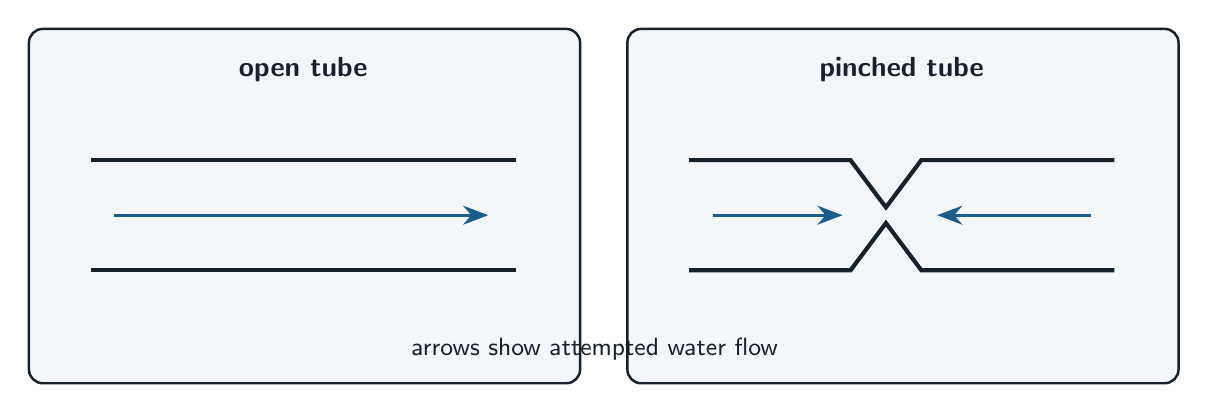
\begin{tikzpicture}[fc text, x=1cm, y=1cm]
  \node[fc panel, minimum width=70mm, minimum height=45mm, anchor=south west] at (0,0) {};
  \node[fc panel, minimum width=70mm, minimum height=45mm, anchor=south west] at (7.6,0) {};
  \node[fc label] at (3.5,4.0) {open tube};
  \node[fc label] at (11.1,4.0) {pinched tube};
  \draw[draw=fcink, line width=1.5pt] (0.8,2.85)--(6.2,2.85) (0.8,1.45)--(6.2,1.45);
  \draw[fc arrow] (1.1,2.15)--(5.85,2.15);
  \draw[draw=fcink, line width=1.5pt]
    (8.4,2.85)--(10.45,2.85)--(10.9,2.25)--(11.35,2.85)--(13.8,2.85)
    (8.4,1.45)--(10.45,1.45)--(10.9,2.05)--(11.35,1.45)--(13.8,1.45);
  \draw[fc arrow] (8.7,2.15)--(10.35,2.15);
  \draw[fc arrow] (13.5,2.15)--(11.55,2.15);
  \node[fc note] at (7.2,0.45) {arrows show attempted water flow};
\end{tikzpicture}
\end{document}
